\chapter{Topological Persistence and Persistent Homology}
\graphicspath{ {/home/tomasp/Dokumenty/Master_Thesis/figures/} }

The \textit{Niyogi-Smale-Weinberger} theorem tells us that it is possible to hope to recover the underlying topology and structure of the space from a limited number of samples from some experiment or study when the distance between the samples is smaller than what is referred to as its \textit{feature scale}.

The problem now lies in finding this feature scale of the object, since this is usually unknowable in advance outside of simulations. Simultaneously, limiting ourselves to looking for a single value of $\varepsilon$ is not the right path either. Some features of the object may become visible for different values of $\varepsilon$, i.e., regions may connect at smaller distances and holes may be created at larger ones. Neither of the two is intrinsically more valuable than the other without additional context. As such, this should motivate us to instead look at multiple feature scales at once and observe the changes in the homology groups for a range of values of $\varepsilon$. Features that exist for a wider range of values are more likely to be more informative about the underlying structure than features that only live for short intervals.

\begin{figure}[h!]
  \centering
  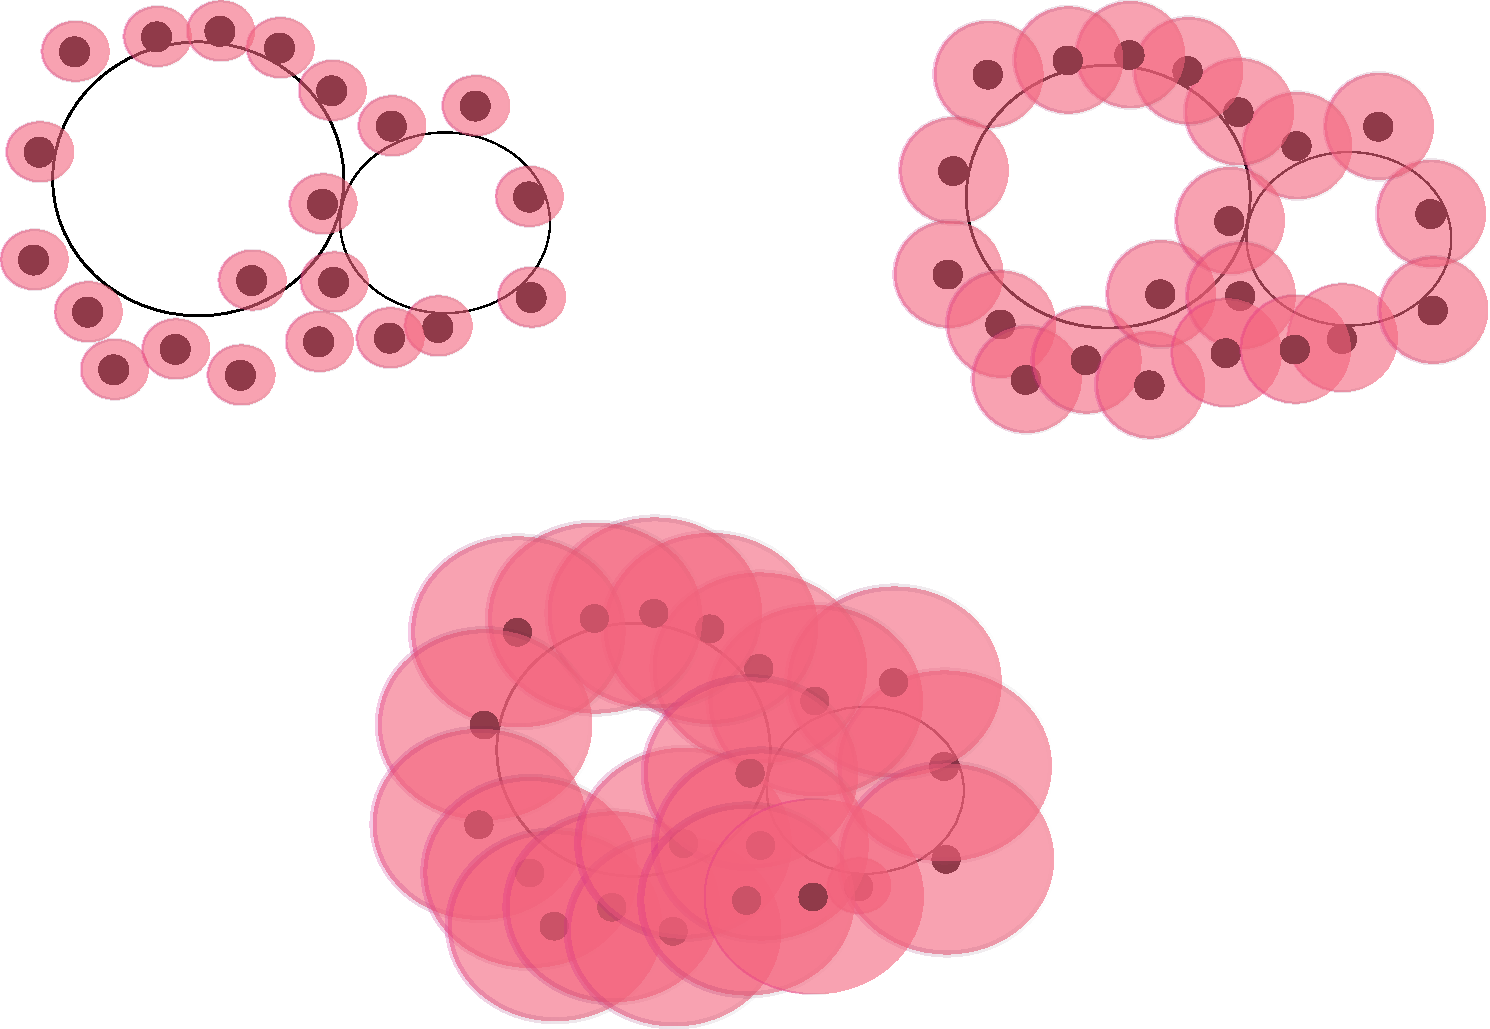
\includegraphics[width=9cm, height=6cm]{filtration_01.pdf}
  \caption{A random sample of points from two touching circles and the growing sublevel sets of the distance function to the points.}
  \label{fig:filtration_01}
\end{figure}

We can consider the point cloud $P$ in \ref{fig:filtration_01} sampled from a curve. Ideally, the goal would be to confirm the existence of one connected component, the two circles touching together, and the presence of two holes, i.e., two loops in total. Even better, we would like to see that one loop is larger and more prominent than the other. This is what the main tool of our work captures -- \textit{persistent homology}.

If we consider the distance function $r: \mathbb{R}^{2} \to \mathbb{R}$, where $r(x) = d(x, P)$, the minimum distance of $x$ to the points in $P$. Taking a look at the sublevel sets of $r$, $r^{-1}[-\infty, a]$ for some $a \in \mathbb{R}^{+} \cup \{0\}$. In this instance, the sublevel sets are unions of closed balls of radius $a$ with the center being the points. By increasing the $a$ from $0$ to infinity, numerous holes will appear, but only the two large loops will live longer than the rest until the entirety of $P$ is covered.

The idea is to translate this rate of survival on the level of points to the survival of individual homology classes whenever we increase the sublevel sets. This is robust since topological ``noise'' dies out quickly in comparison to the interesting topological features. Persistent homology effectively takes a function defined on the topological space and observes the evolution of homology classes over increasing sublevel sets of the function.

It should be noted that there are two different scenarios where persistence takes place. One is where our function is defined on a topological space, which would require the use of singular homology; previously established to be computationally intractable. The other, the one we are interested in, is the case where the function is defined on a simplicial complex. The sequence of sublevel sets there is simply the nested sequence of subcomplexes, usually referred to as a \textit{filtration}. Naturally, here we will be working with simplicial homology, which we know how to efficiently compute.

\subsection{Filtration and persistence}
\subsubsection{Topological spaces}

Let $f: \mathbb{T} \to \mathbb{R}$ be a function defined on a topological space $\mathbb{T}$. If we denote $\mathbb{T}_{a} = f^{-1}(-\infty, a]$, the sublevel set of the function $f$ for the value $a$, then certainly this inclusion holds:
  \begin{equation*}
    \mathbb{T}_{a} \subseteq \mathbb{T}_{b} \quad \text{for}\: a \leq b.
  \end{equation*}

  The point is to consider a sequence of real numbers $a_{1} \leq a_{2} \leq \ldots \leq a_{n}$ to create a sequence of nested subspaces of $\mathbb{T}$

  \begin{figure}[h]
    \centering

    \begin{tikzcd}
      \mathcal{F}_{f}: \varnothing = \mathbb{T}_{a_{0}} \arrow[r, hook] & \mathbb{T}_{a_{1}} \arrow[r, hook] & \mathbb{T}_{a_{2}} \arrow[r, hook] & \ldots \arrow[r, hook] & \mathbb{T}_{a_{n}}
    \end{tikzcd}

  \end{figure}

  We call this sequence a \textit{filtration} $\mathcal{F}_{f}$. Ideally, the points $a_{1} \leq \ldots \leq a_{n}$ would be where the homology groups of the sublevel sets go through some change, i.e., new features are born or old ones die. Realistically speaking, we usually cannot hope to guess those values \textit{apriori} and are forced to iterate over a much larger range of admissible values.

  The inclusion maps between each sublevel set induce a linear map in the singular homology groups (since we consider general topological spaces). Denoting $\iota: \mathbb{T}_{a_{i}} \to \mathbb{T}_{a_{j}}$, $i \leq j$, the inclusion map $x \mapsto x$, we have an induced homomorphism

  \begin{equation*}
    h_{p}^{i,j} = \iota_{*}: H_{p}(\mathbb{T}_{a_{i}}) \to H_{p}(\mathbb{T}_{a_{j}})
  \end{equation*}
  for all $p \geq 0$, $0 \leq i \leq j \leq n$. Doing this, we tranform the nested sublevel sets into a structure we call a \textit{homology module}:

  \begin{figure}[h]
    \centering
    \begin{tikzcd}
      0 = H_{p}(\mathbb{T}_{a_{0}}) \arrow[r, hook] & H_{p}(\mathbb{T}_{a_{1}}) \arrow[r, hook] & H_{p}(\mathbb{T}_{a_{2}}) \arrow[r, hook] & \ldots \arrow[r, hook] & H_{p}(\mathbb{T}_{a_{n}}).
    \end{tikzcd}
  \end{figure}
